\chapter{Guía de mantenimiento de Arch Linux}
\label{chap:archlinux_maintenance_guide}

\lettrine{E}{n} este apéndice se encuentra una breve guía de los comandos más básicos para mantener Clúpiter a punto, especialmente haciendo enfoque en las actualizaciones y mantenimiento básico del sistema.

\section{Enlaces de interés}
Ante cualquier duda, consulta, o problema, se debe acudir a la wiki de Arch Linux, donde lo más probable es que se encuentre la respuesta. A continuación se muestra una lista de entradas relevantes de esta wiki y similares:

\begin{itemize}
    \item Introducción a Arch Linux, donde en especial se recomienda la sección ``Package management'':
    \url{https://wiki.archlinux.org/title/General_recommendations}.

    \item Arch User Repository. Este es un repositorio gestionado por la comunidad, donde se pueden encontrar gran cantidad de paquetes no soportados oficialmente, pero que habitualmente cuentan con un soporte de calidad. En caso de emplearse de forma asidua, se recomienda instalar un \textit{wrapper} de AUR, como por ejemplo \texttt{yay} o \texttt{paru}:\\
    \url{https://wiki.archlinux.org/title/Arch_User_Repository}.

    \item Manual para systemd: \url{https://wiki.archlinux.org/title/Systemd}.
    \item Configuración de red: \url{https://wiki.archlinux.org/title/Systemd-networkd}.
    \item Configuraciones para \acrlong{rpi}: \\\url{https://archlinuxarm.org/wiki/Raspberry_Pi}.

    \item Manual de pacman, el gestor de paquetes de Arch Linux: \\\url{https://wiki.archlinux.org/title/General_recommendations}.
\end{itemize}

Para un usuario más novato esto podría parecer abrumador en un principio, pero desde mi punto de vista esta es la mejor forma de aprender, y el espíritu que promueve Arch Linux. 

\section{Actualización del sistema}
Si se han leido con detenimiento las entradas en la sección anterior no debería haber mucha duda en qué hacer para actualizar el sistema. Sin embargo, siempre vienen bien las recomendaciones basadas en la experiencia.

Como Clúpiter probablemente se actualice muy de vez en cuando, es necesario tomar precauciones para evitar posibles comportamientos indeseados tras la actualización. De esta forma, estando conectados a internet, y por este orden, se debe ejecutar en todos los nodos:

\begin{enumerate}
    \item Hacerse superusuario.
\begin{lstlisting}[language=bash]
su -
\end{lstlisting}
    \item Actualizar la base de datos de pacman:
\begin{lstlisting}[language=bash]
pacman -Syy
\end{lstlisting}
    \item Actualizar los llaveros de claves, o \textit{keyring}:
\begin{lstlisting}[language=bash]
pacman -S archlinux-keyring archlinuxarm-keyring
\end{lstlisting}
    \item Visualizar el resto de actualizaciones con:
\begin{lstlisting}[language=bash]
pacman -Syu
\end{lstlisting}
    \textbf{NOTA:} Los servidores de ArchLinuxARM no parecen ser los mejores, por lo que a veces puede dar error al descargar algún archivo. En ese caso, no hay de qué preocuparse: \texttt{pacman -Syu} es idempotente, y se puede ejecutar todas las veces requeridas hasta que se descarguen todos los paquetes. Aún así, es conveniente esperar un pequeño tiempo por si el servidor está experimentando dificultades técnicas transitorias.
    
    \item Verificar las versiones de las actualizaciones, \textbf{especialmente las que cambien de versión mayor}, esto es, de php 7 a php 8, por ejemplo. Si hubiera alguna actualización mayor, es conveniente hacer una búsqueda en internet para verificar que no haya incompatibilidades.
    Por ejemplo, en el caso de php, se buscaría ``php 8 update arch linux'', y entre los primeros resultados se encuentra: \\\footnotesize\url{https://archlinux.org/news/php-80-and-php-7-legacy-packages-are-available/}\normalsize

    Además, es muy conveniente verificar las noticias en la sección principal de \url{https://archlinux.org}, donde suelen dar la solución a los problemas que se puedan encontrar durante la actualización, especialmente en el caso de que algún paquete sea eliminado, sustituído por otro, o haya algún problema de dependencias derivado de las situaciones anteriores.

    \item Finalmente, proceder y realizar la actualización pulsando \texttt{Y}, \texttt{S}, o \texttt{<ENTER>} (esta última acepta la letra en mayúscula, lo cual es habitualmente la mejor idea). Es recomendable reiniciar tras una actualización del kernel, lo cual es algo probable si éstas se realizan cada bastante tiempo.
\end{enumerate}

\subsection{Asciinema}
En la dirección \url{https://asciinema.org/a/434085}, se puede ver el proceso de actualización de uno de los nodos de Clúpiter. Recordar que esta acción debe llevarse a cabo simultáneamente en todos los nodos, por ejemplo, activando la difusión al grupo con el programa terminator, como se ve en la Figura \ref{fig:terminator_update}. Además, el archivo grabado se puede encontrar en el repositorio del proyecto bajo la carpeta \texttt{doc/asciinema}, y se puede reproducir con el comando \texttt{asciinema play archlinux-update.cast}.

\begin{figure}[h!]
  \centering
  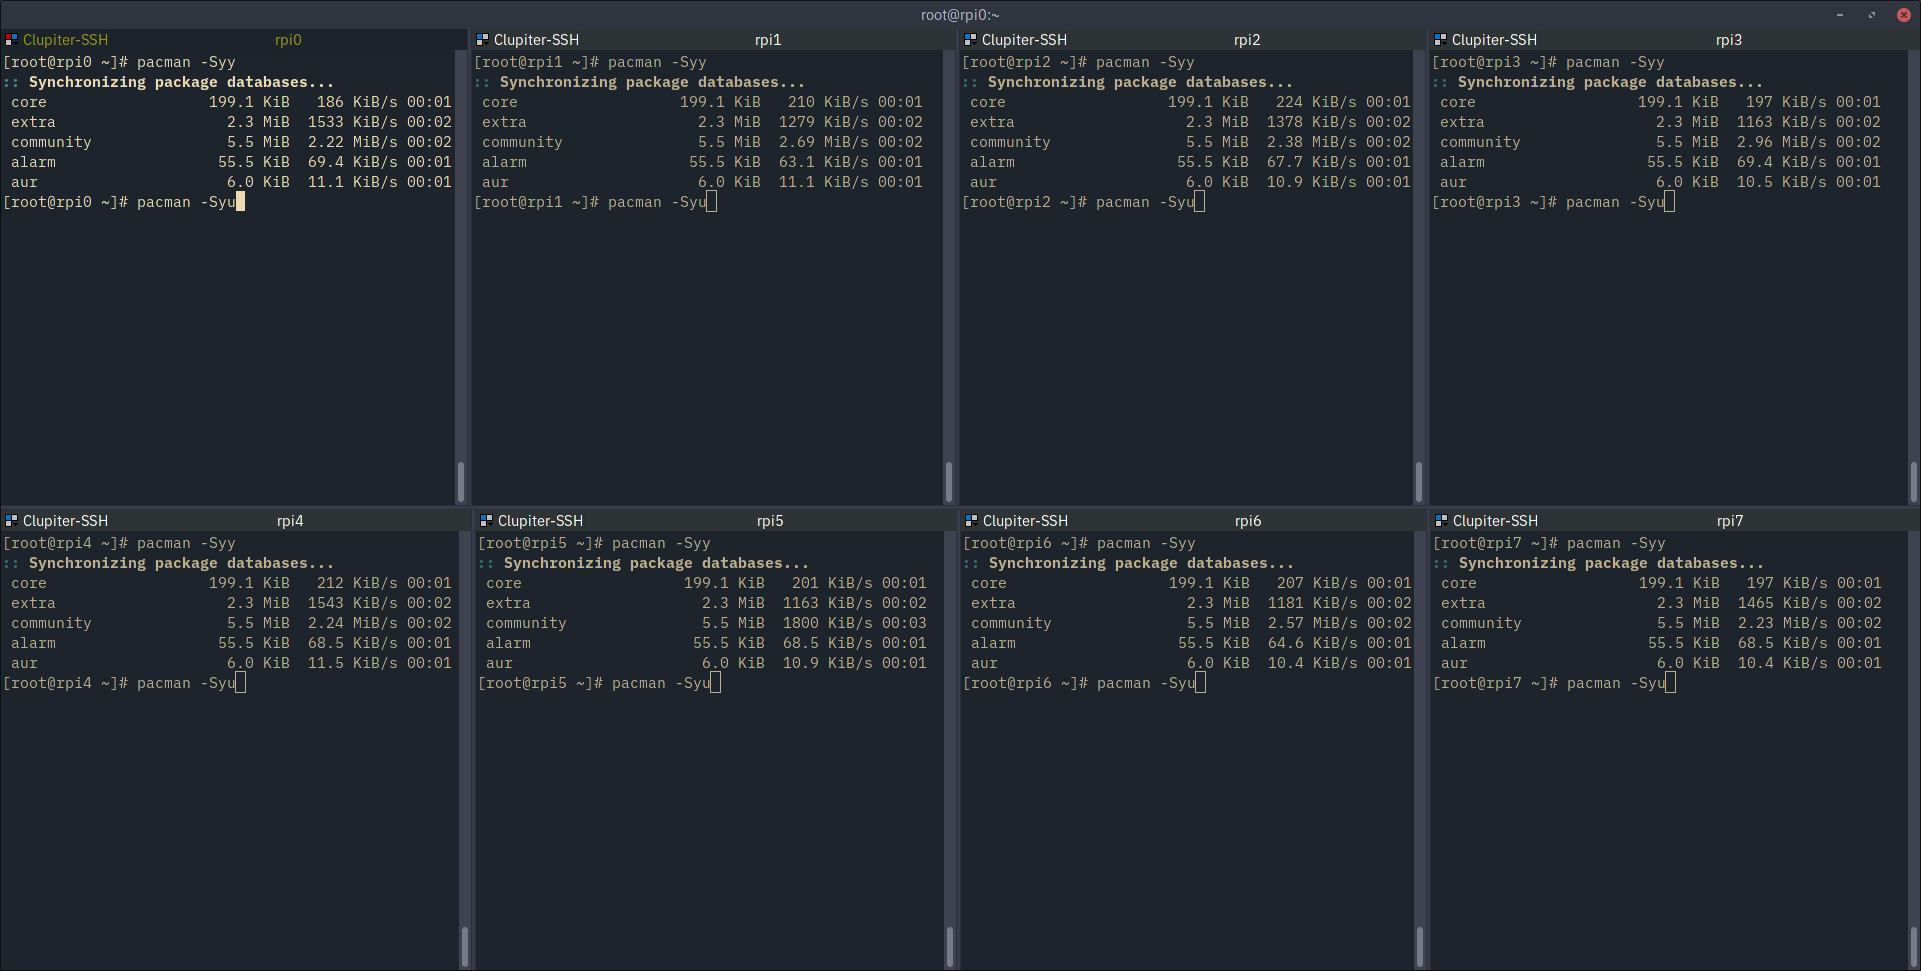
\includegraphics[width=\textwidth]{img/terminator_update.png}
  \caption{Operación en paralelo de Clúpiter con terminator}
  \label{fig:terminator_update}
\end{figure}